% !TEX encoding=utf8
\documentclass[10pt,a4paper]{scrartcl}

\usepackage{ucs}
\usepackage[utf8]{inputenc}
\usepackage[ngerman]{babel}
\usepackage{amsmath}
\usepackage{amssymb, amstext}
\usepackage{mathtools}
\usepackage[pdftex]{graphicx}
\usepackage{bibgerm}
\usepackage{amsthm}
\usepackage[colorlinks=true]{hyperref}
\usepackage{dsfont}
\usepackage{caption}
\usepackage{multicol}
\usepackage{pdfpages}
\usepackage[a4paper,left=2.5cm,right=2.5cm,top=2cm,bottom=4cm,bindingoffset=5mm]{geometry}
\usepackage{tikz}
%\usepackage{txfonts}
\usepackage{textcomp}
\usepackage{multirow}
\pagestyle{headings}
\usepackage{tabularx}
\usepackage{enumerate}
\newcolumntype{L}[1]{>{\raggedright\arraybackslash}p{#1}} % linksbündig mit Breitenangabe
\newcolumntype{C}[1]{>{\centering\arraybackslash}p{#1}} % zentriert mit Breitenangabe
\newcolumntype{R}[1]{>{\raggedleft\arraybackslash}p{#1}} % rechtsbündig mit Breitenangabe
\usepackage{subfig}

\setlength{\topmargin}{-15mm}
%\setcounter{secnumdepth}{5} %wie viele Level


%\usepackage[latin1]{inputenc}
\usepackage[T1]{fontenc}
%\usepackage{ae,aecompl}
%\usepackage{amsmath,amssymb,amstext}
\usepackage{psfrag}
\usepackage{caption}
\usepackage{booktabs}
\usepackage{tabularx}
\captionsetup[table]{textfont=it,justification=raggedright,singlelinecheck = false}
\usepackage{float}




%%%%

% einige Abkuerzungen
\newcommand{\C}{\mathbb{C}} % komplexe
\newcommand{\K}{\mathbb{K}} % komplexe
\newcommand{\R}{\mathbb{R}} % reelle
\newcommand{\Q}{\mathbb{Q}} % rationale
\newcommand{\Z}{\mathbb{Z}} % ganze
\newcommand{\N}{\mathbb{N}} % natuerliche

%Zum markieren: http://texwelt.de/wissen/fragen/2803/wie-kann-ich-formel-teile-einer-gleichung-einkreisen
\newcommand\mrahmen[3][]{%
  \tikz[anchor=base,baseline]\node[inner sep=2pt,draw=#2,#1]{$\displaystyle#3\mathstrut$};}
\colorlet{mfarbe}{red}


%verschiednen sachen die man mit begin{...} dann einzeln durchnummerrienen lassen kann
\newtheorem{defin}{Definition}
\newtheorem{satz}{Satz}
\newtheorem{formel}{Formel}
\newtheorem{abbildung}{Abbildung}
\newtheorem{versuch}{Versuch}


%Titel Gedöns
\title{Versuch F09\\ Neuromorphic Computing}
\date{Lab book}
\author{Xeno Boecker, Jan Jakob}
\date{}

\begin{document}


\pagenumbering{roman} %% small roman page numbers

%%% include the title
\thispagestyle{empty}  %% no header/footer (only) on this page
 \maketitle

%%% start a new page and display the table of contents
\newpage
\tableofcontents

%%% start a new page and display the list of figures
%\newpage
%\listoffigures

%%% start a new page and display the list of tables
%\newpage
%\listoftables

%%% display the main document on a new page 
\newpage

\pagenumbering{arabic} %% normal page numbers (include it, if roman was used above)


\section{Investigating a Single Neuron}

In the first experiment, we will investigate the firing behavior of a single neuron without input. The neuron can be brought into a continuous firing regime by setting the leakage reversal potential above
the firing threshold.

\subsection{Task 1}
In fhe following we draw an equivalent circuit of a neuron in the described configuration. Therefore, we take the neuron schematic in Figure 5 as a reference. 

\begin{figure} [ht]
\begin{center}
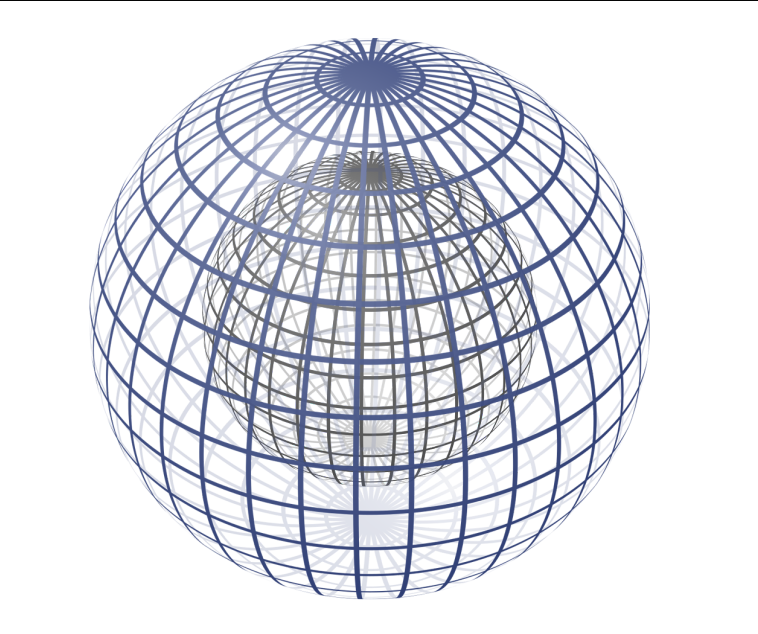
\includegraphics[scale=0.1]{pictures/example.png}
\caption{equivalent circuit of a neuron in the described configuration}
\label{fig:schaltung1}
\end{center}
\end{figure}

\noindent \textbf{Question:} Which parameters of the neuron will influence to the firing frequency? 


\subsection{Task 2}
In this task we did only computational preparation.


\subsection{Task 3}
Look at the generated plot and verify that the values for threshold voltage V th and reset



voltage E r are set correctly.


\subsection{Task 4}


\newpage



\section{Calibrating Neuron Paramters}


\subsection{Task 1}

\subsection{Task 2}

\subsection{Task 3}

\subsection{Task 4}

\subsection{Task 5}



\end{document}
